\begin{frame}{Quadrilateral exercise}
\begin{enumerate}
\conti
\item ABCD is a rhombus and P, Q, R and S are the
mid-points of the sides AB, BC, CD and DA
respectively. Show that the quadrilateral PQRS
is a rectangle.
\seti
\end{enumerate}
\textbf{Solution:}
\begin{itemize}
\item Construct a rhombus wih following coordinates $$A=\begin{pmatrix}
0 \\3 
\end{pmatrix},
B=\begin{pmatrix}
5 \\0 
\end{pmatrix},
C=\begin{pmatrix}
0 \\3
\end{pmatrix},
D=\begin{pmatrix}
-5 \\0 
\end{pmatrix}$$
\item Find P,Q,R,S
\item $P=\frac{(A+D)}{2},Q=\frac{(D+C)}{2},R=\frac{(C+B)}{2} and S=\frac{(A+B)}{2}$
\end{itemize}
\end{frame}
\begin{frame}
\begin{figure}[!h]
\resizebox{0.5\linewidth}{!}
{
\begin{tikzpicture}[scale =2.5,>=stealth,point/.style = {draw, circle, fill = black, inner sep = 2pt},]
\node (A) at (0,-3)[point,label=below :$\textbf{A(0,-3)}$] {};
\node (B) at (5,0)[point,label=above :$\textbf{B(5,0)}$] {};
\node (D) at (-5,0)[point,label=below :$\textbf{D(-5,0)}$] {};
\node (C) at (0,3)[point,label=above :$\textbf{C(0,3)}$] {};
\node (S) at (-2.5,-1.5)[point,label=above left :$\textbf{S(-2.5,-1.5)}$] {};
\node (R) at (-2.5,1.5)[point,label=above left :$\textbf{R(-2.5,1.5)}$] {};
\node (Q) at (2.5,1.5)[point,label=above right :$\textbf{Q(2.5,1.5)}$] {};
\node (P) at (2.5,-1.5)[point,label=below right :$\textbf{P(2.5,-1.5)}$] {};
\draw (A) --(B)--(C)--(D)--(A);
\draw (P) --(Q)--(R)--(S)--(P);
\draw (Q) --(S);
\draw (P) --(R);
\draw (A) --(C);
\draw (B) --(D);
\tkzMarkAngle[fill=black!45,size=.3,mark=](S,P,A)
\tkzLabelAngle[pos=-0.55](S,P,A){$\angle{3}$}
\tkzMarkAngle[fill=blue!45,size=.3,mark=](B,P,Q)
\tkzLabelAngle[pos=0.45](B,P,Q){$\angle{1}$}
\tkzMarkAngle[fill=red!45,size=.3,mark=](P,Q,B)
\tkzLabelAngle[pos=0.45](P,Q,B){$\angle{2}$}
\tkzMarkAngle[fill=green!45,size=.3,mark=](C,Q,R)
\tkzLabelAngle[pos=0.45](C,Q,R){$\angle{4}$}
\end{tikzpicture}


}
\caption{tikz figure}
\label{fig:foo}
\end{figure}
\end{frame}
\begin{frame}
\begin{figure}[!h]
\resizebox{0.3\linewidth}{!}
{
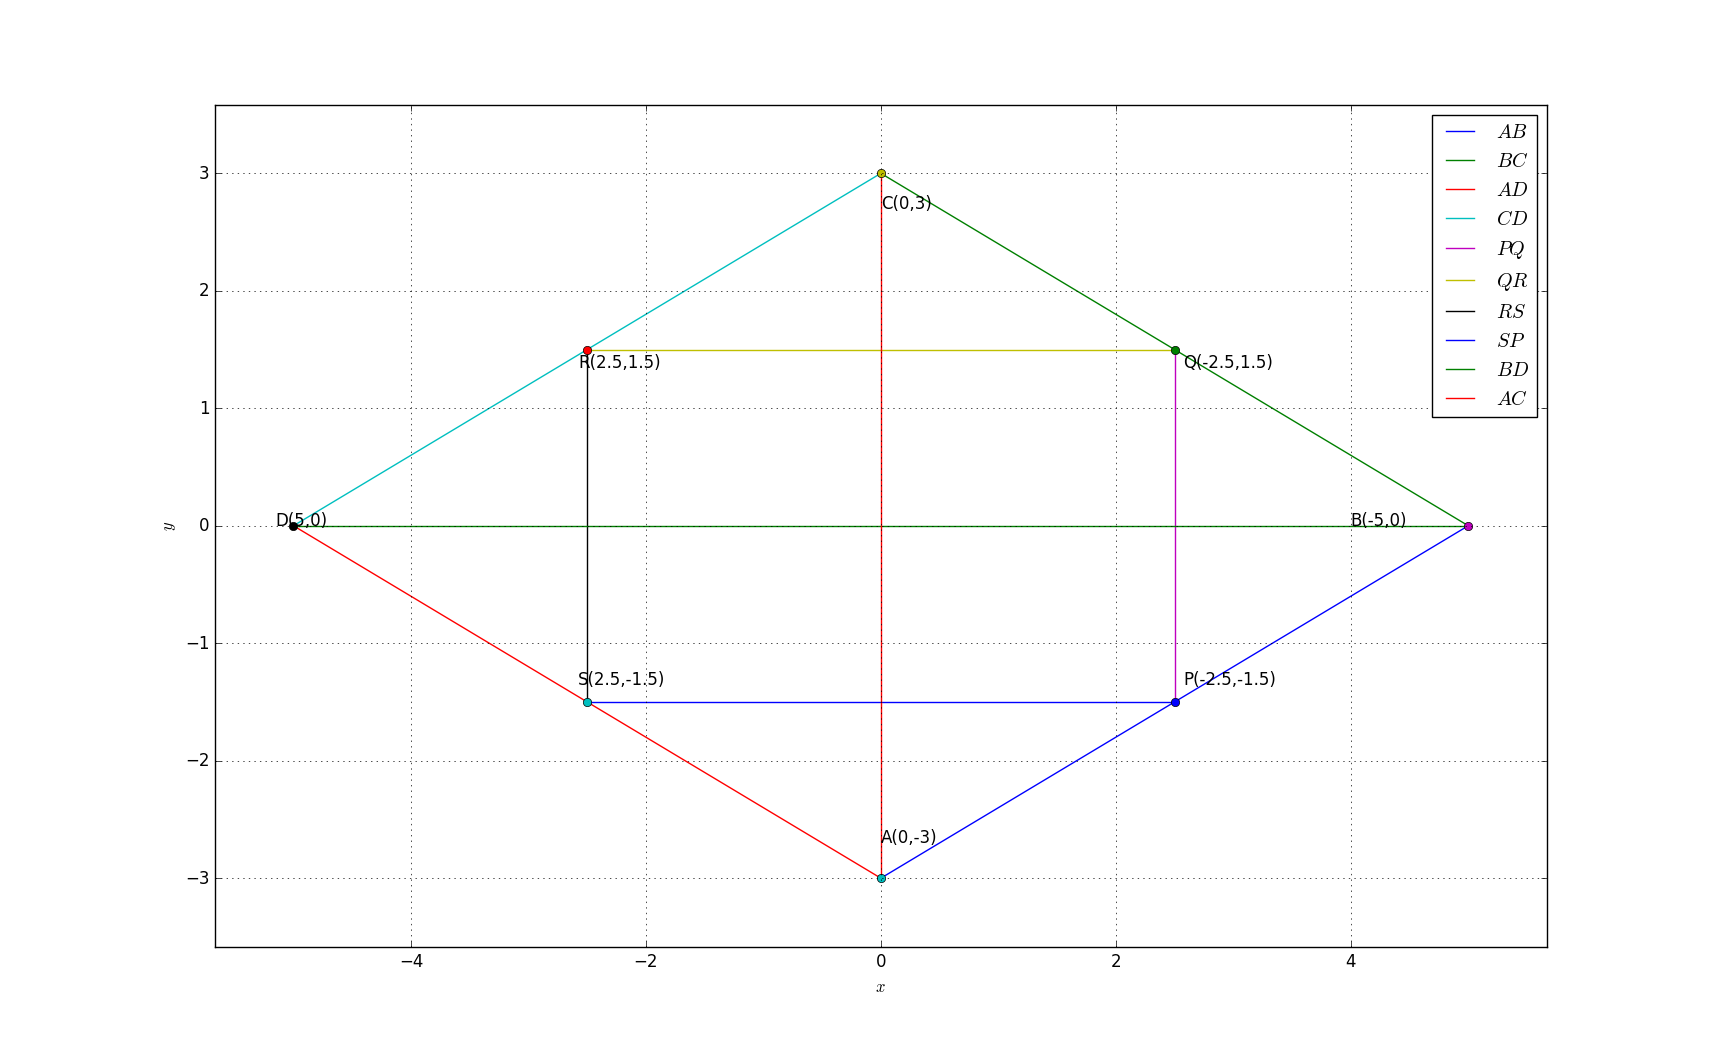
\includegraphics[scale=1.2]{./figs/quad/rhomb.png}

}
\caption{Rhombus}
\label{fig:foo}
\end{figure}
From $\triangle{ABC}$ and $\triangle{ADC}$
\begin{align}
PQ || AC \hspace{2pt}\text{and}\hspace{2pt} PQ=\frac{1}{2}AC\\
RS || AC \hspace{2pt}\text{and}\hspace{2pt} RS=\frac{1}{2}AC
\end{align}
from 11 and 12 PQ=RS , PQ||RS 
\begin{align}
 \textit{As}\hspace{6pt} PB=PQ, \angle{2} =\angle{1}
\end{align}
From $\triangle{APS}$ and $\triangle{CQR}$ \\
\begin{itemize}
\item AP=CQ,AS=CR, PS=QR\\
\item From SSS rule
$\triangle{APS} \cong \triangle{CQR}$
\begin{align}
\angle{3} = \angle{4}
\end{align}
\end{itemize}
\end{frame}
\begin{frame}
For AB, BC
\begin{align}
\angle{3}+\angle{SPQ}+\angle{1} = 180\degree
\end{align}
\begin{align*}
\angle{2}+\angle{PQR}+\angle{4}=180\degree
\end{align*}
from 13 and 15 
\begin{align}
\angle{1}+\angle{PQR}+\angle{3}=180\degree
\end{align}
\begin{center}
PS|| PR $\angle{SPQ}+\angle{PQR} =180\degree \implies \angle{SPQ}=90\degree$
\end{center}
tikz : \url{https://github.com/d-DP/geometryy/blob/master/figs/quad/quad_exer.tex}\\
python : \url{https://github.com/d-DP/geometryy/blob/master/codes/quad/rhombus.py}
\end{frame}